\documentclass[11pt]{report}
\usepackage[pdftex]{graphicx}

\usepackage{henrian-basic}
\usepackage{henrian-homework}

\usepackage{amsmath}
\usepackage{float}

\makeHeaders{Machine Learning: Homework 6}

\begin{document}

\begin{itemize}
  \item \textbf{Email}: chrisbrown@utexas.edu
  \item \textbf{EID}: chb595
\end{itemize}

\section{Bayes Nets}

The actual network in this homework was small but not trivial. It had nodes without parents, nodes with multiple children, and nodes with multiple parents. What was simple, though, was that each node produced a boolean value. This means that the graph had just 10 total parameters to be learned.

The goal of the homework was to be able to marginalize out any single node using Gibbs sampling. Even though exact inference is easy and fast, the Gibbs sampling approach here would be applicable in other situations where: 1) the parameters of the original distributions are unknown, or 2) the graph is very large and exact inference is computationally intractable (or simply overkill).

On my very first run-through, I forgot to set the $Z_i$ of my $Z$ vector to the new value on each draw. This was confusing, because the algorithm still produced a decent result more than half the time, and the other times, it was exactly the opposite ($1 - exactInf$) of what the result should have been. That was an obvious error, though; after fixing it, that behavior disappeared.

A naive first implementation worked surprisingly well; at 1,000 iterations and no burn-in, the results are still pretty good:

\begin{figure}[H]
  \centering
  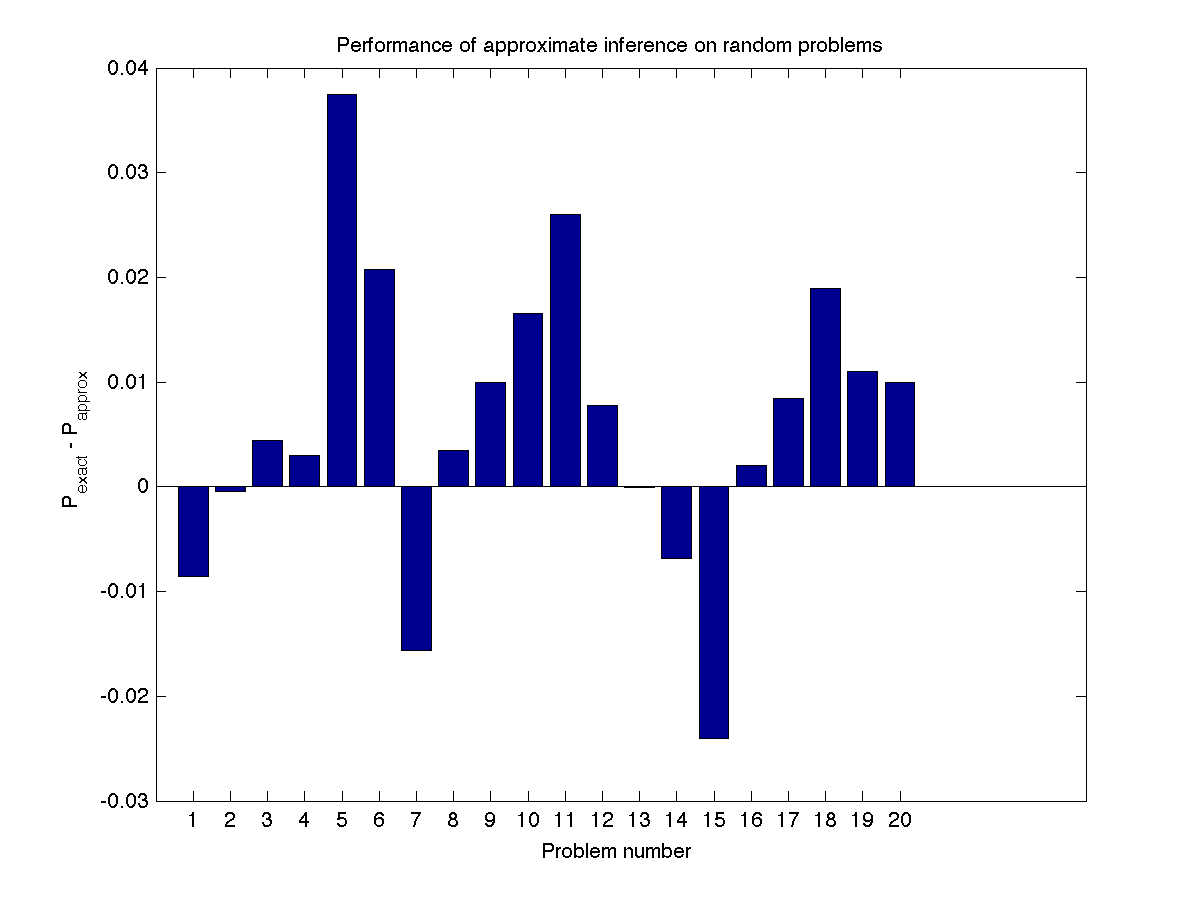
\includegraphics[width=0.8\textwidth]{hw6-plot-n1000.png}
  \caption{Accuracy (nearness to exact inference result) for 1,000 iterations.}
  \label{fig:n1000}
\end{figure}

\noindent Simply by taking 10x samples, still without a burn-in period, we get much better results:

\begin{figure}[H]
  \centering
  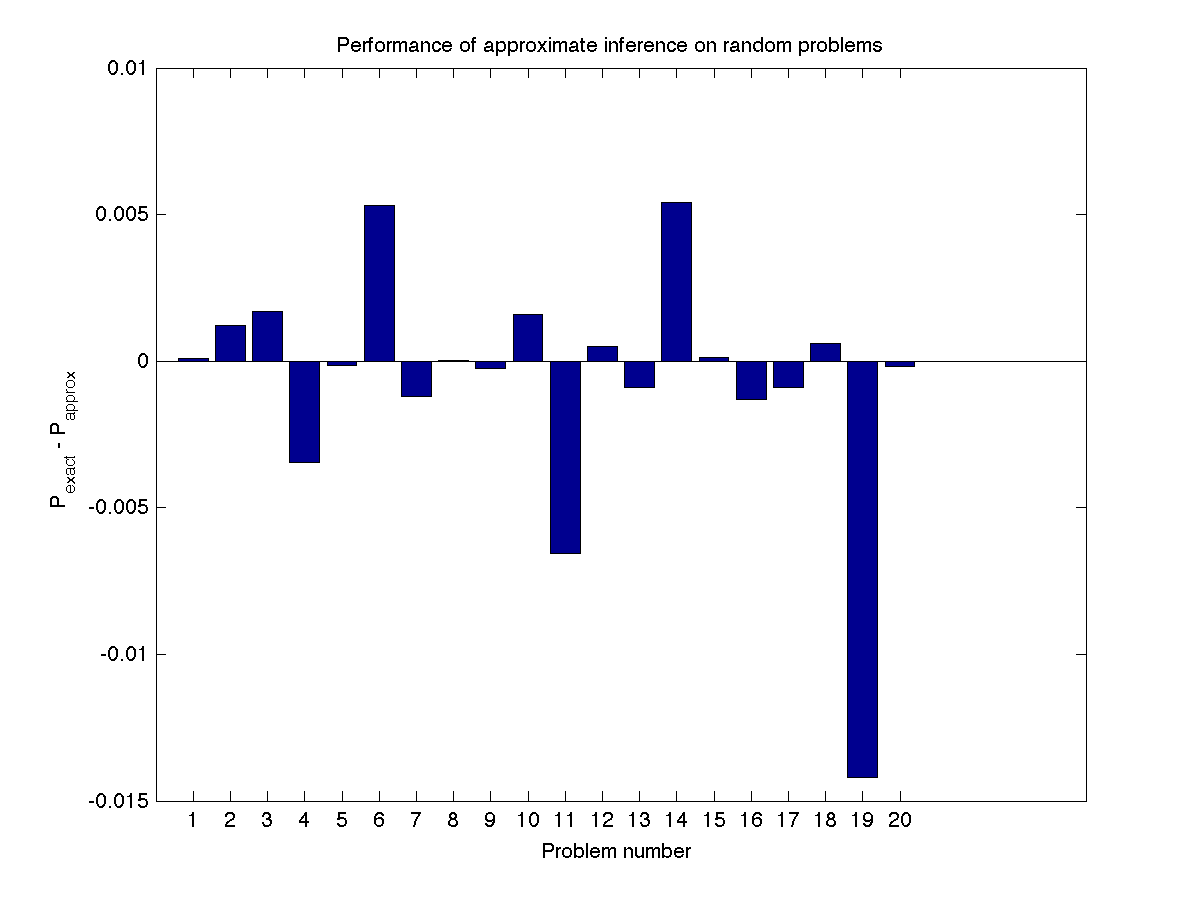
\includegraphics[width=0.8\textwidth]{hw6-plot-n10000.png}
  \caption{Accuracy (nearness to exact inference result) for 10,000 iterations.}
  \label{fig:n10000}
\end{figure}

\noindent In Figure \ref{fig:n10000}, Sample 19 is a lot further off than we might like. Allowing a burn-in period of $1/10$ the total number of iterations gets us to the next plateau of accuracy:

\begin{figure}[H]
  \centering
  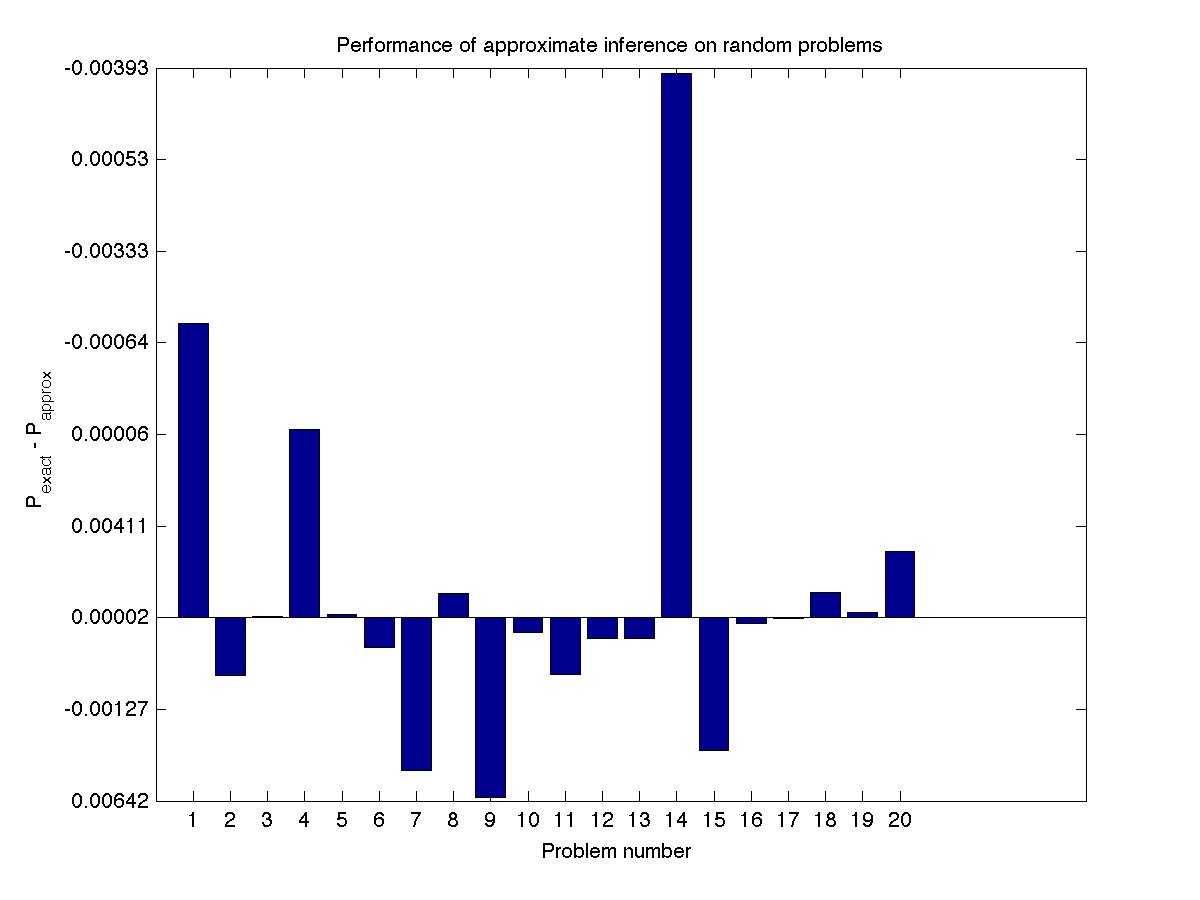
\includegraphics[width=0.8\textwidth]{hw6-plot-n10000-burnin.png}
  \caption{Accuracy (nearness to exact inference result) for 10,000 iterations, allowing for 1,000 iterations of burn-in.}
  \label{fig:n10000-burnin}
\end{figure}

\section{Comments}

I'm still curious why I didn't have to (or get to) use the intermediate results from samples as part of the sampling process. Just to restate what I asked in my email, and provide a little elaboration: since we're drawing from an artificial distribution, for which we know the exact parameters at every node, there's no apparent reason how we could possibly do better. However, in the MCMC and Gibbs Sampling tutorial (EEB 581 lecture notes\footnote{http://web.mit.edu/\~wingated/www/introductions/mcmc-gibbs-intro.pdf}), their example implementation of the algorithm shows them updating the priors upon each new draw/sample (p. 17, in Ex. 4, step (ii) and elsewhere), which is straightforward in that case because they are using Binomial and Beta distributions, which have very simple updates.

To do this for this homework, I would have had to extract the functionality of the \texttt{computeJoint(...)} function, digging down into the actual CPD's for each draw, and adding my current number of successes and observations to the parameters/priors as needed.

I think that the reason why they do this in the tutorial is in case you're drawing from a real distribution that you don't know the parameters. If you only have a list of observations, 


\end{document}
